\documentclass[11pt,twoside,titlepage]{article}
\usepackage[tc]{titlepic}
\usepackage{times}
\usepackage{float}
\usepackage{amssymb}
\usepackage{amsmath}
\usepackage{amsthm}
\usepackage{needspace}
\usepackage{url}
\usepackage{hyperref}
%\usepackage{mathptm}
\usepackage{fancyhdr}
\usepackage{wrapfig}
\ifx\pdfoutput\undefined
% we are running LaTeX, not pdflatex
\usepackage{epsfig,color}
\else
% we are running pdflatex, so convert .eps files to .pdf
\usepackage[pdftex]{epsfig,color}
\usepackage{epstopdf}
\usepackage{pdfsync}
\fi
\usepackage{ifthen,version}
\usepackage{listings}
%\usepackage{temporal}
%\usepackage{algorithmic}
\newboolean{print-solutions}

% Start of configuration section
% Comment out the following line to exclude the printing of solutions.
%\setboolean{print-solutions}{true}
\newcommand{\labnumber}{1}
\newcommand{\labname}{Digital Logic Gates}
\newcommand{\coursenumber}{Circuit Basics How-To Document}
\newcommand{\coursename}{Introduction to Digital Design}
% End of configuration section

% Conditional definitions
\newcommand{\dateorsol}{\LARGE \ifthenelse{\boolean{print-solutions}}%
  {Solutions}{Due \duedate}}
\newcommand{\headertxt}{\sl \ifthenelse{\boolean{print-solutions}}%
  {Solutions to}{} Laboratory Exercise \#\labnumber}
\newcommand{\points}[1]{\ifthenelse{\boolean{print-solutions}}%
  {}{[#1 points.]}}
\ifthenelse{\boolean{print-solutions}}{\includeversion{prnt-solns}}%
{\excludeversion{prnt-solns}}

\textwidth=7.25in
\evensidemargin=-0.35in
\oddsidemargin=-0.35in

\newcommand{\ite}{\operatorname{ite}}
\newcommand{\itec}{\operatorname{ite\_constant}}

{\theoremstyle{definition} \newtheorem{definition}{Definition}}
\newtheorem{theorem}{Theorem}
\newtheorem{lemma}{Lemma}
\newtheorem{corollary}{Corollary}
\newtheorem{proposition}{Proposition}
{\theoremstyle{remark}
  \newtheorem{example}{Example}
  \newtheorem{problem}{Problem}
  \newtheorem{note}{Note}}
% Fortunately, proofs can be nested.
\newenvironment{solution}{\begin{proof}[Solution]}{\end{proof}}


\newcommand{\ta}{Created By: Kyler Scott and Prof. Sunil P. Khatri\\July 2020}
\title{ \huge Department of Electrical and Computer Engineering \\ \huge Texas A\&M University}
\author{ \huge Circuits Basics:\\ \\ \huge How-To Document\\ \\ \\ \ta}

\titlepic{
\includegraphics[width=0.5\textwidth]{logo}}

\date{}
\pagestyle{fancy}
\lhead[\rm\thepage]{}
\rhead[]{\rm\thepage}
\lfoot[]{\coursenumber}
%\cfoot{\instructor}
\rfoot[\coursenumber]{}

\begin{document}
\bibliographystyle{alpha}
\maketitle

\noindent
\textbf{Note:} Learning the fundamentals of digital circuits and successfully completing lab assignments will require that you learn to use your lab equipment properly. Before attempting to perform anything in this document, please read the "Lab Safety" document. It contains important information that will teach you to avoid potential hazards such as destroying your lab equipment or even starting a fire.\\

\section{Introduction}
This guide will cover the basics of creating and measuring digital circuits wired on a breadboard.

\section{Bread-boarding Techniques}
The bread-board used in ECEN 248 and ECEN 449/749 is depicted in Figure~\ref{bread_board}. Take a moment to examine it. Here are a few techniques which will help you wire up your circuits:

\begin{enumerate}
	\item Horizontal lines of points on the bread-board are electrically connected together. However, lines are not connected across the partition divisions (i.e. lines in different partition are independent).
	
	\item Vertical lines of points are \textbf{NOT} electrically connected, except in the case of a power or ground line (see Figure~\ref{bread_board}).
	
	\begin{figure}[htpb]
		\centering 
		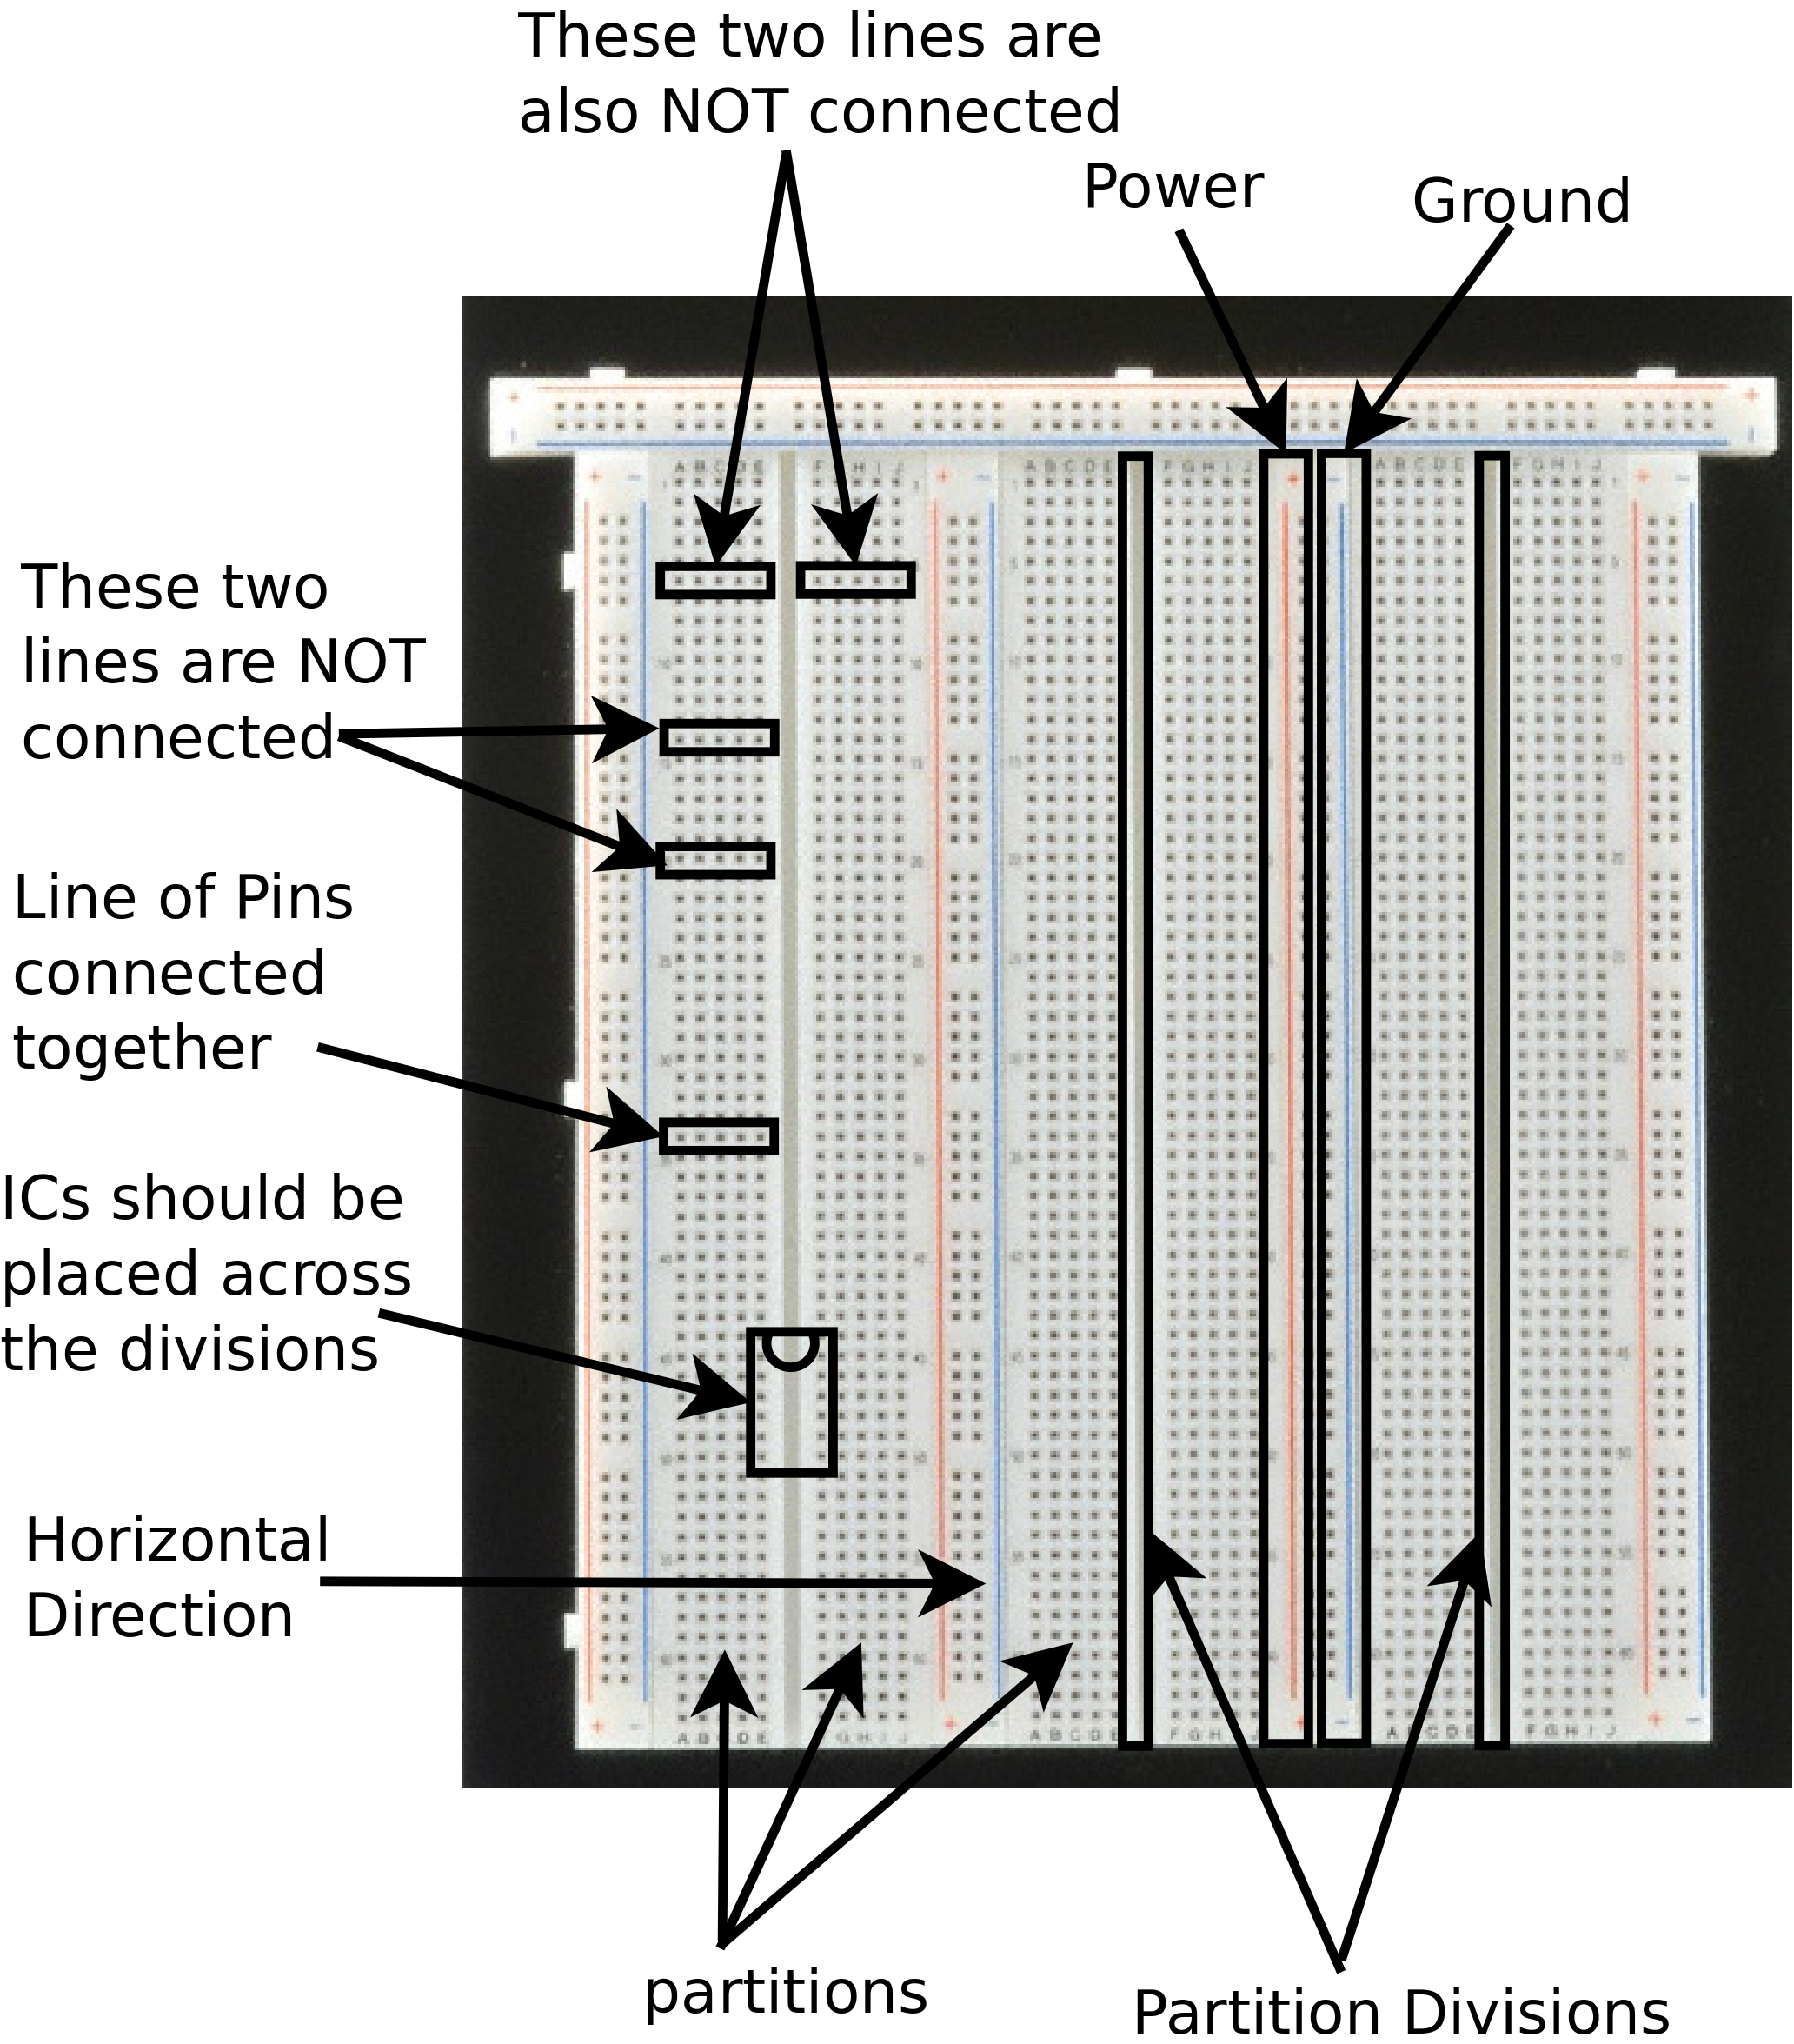
\includegraphics[ width=.9\textwidth]{bread_board}
		\caption{Bread-Board}
		\label{bread_board}
	\end{figure}
	
	\item Power and Ground lines shown vertically in Figure~\ref{bread_board} are electrically connected. In lab, you will connect the 5V supply to one of the pins in the Power line. This will connect the entire column to the 5V supply. Similarly, the Ground signal needs to be connected to one pin in the Ground line.
	
	\item All the Integrated Circuits (ICs) in the design should be placed across one of the partition divisions as shown in Figure~\ref{bread_board}. Do not place an IC in only one partition because this will short pins together causing the IC to burn up.
	
	\item Wires connecting different IC pins should traverse horizontally or vertically \textbf{only}. Do not connect wires diagonally across the breadboard as this will result in a messy design making it difficult to debug.
	
	\item Use smaller wires when connecting nearby points on the breadboard. Please use wire strippers to shorten wires if smaller sized wires are not available. This will help keep your design clean and easy to debug.
	
	\item You may decide to always place the IC in such a way that the notch is located on the top (or bottom) as shown in Figure~\ref{bread_board}. This may help you identify pin numbers. Similarly, it might be a good idea to use color codes while wiring up your design. For example, you could assign black wires to the least significant bit, white wires to the next significant bit, green wires to the next, and red wires for the most significant bit. The color code and order of assignment is entirely your choice and for your convenience in identifying wire connections while debugging.
	
	\item Before placing the components on the breadboard, plan the placement of your ICs such that it minimizes wiring distance on the breadboard. ICs with high connectivity should be placed near each other. For example, if LED display inputs are connected to OR gate outputs, then try to place the OR gate IC as close as possible to the LED display.
\end{enumerate}


\section{Measuring Voltages}

\noindent
In a digital circuit, a voltage on any wire should be at one of two levels: either near 0V (GND) or near VCC. VCC is the supply voltage value, and it can vary. Sometimes it may be equal to 5V (like in ECEN 248 labs), sometimes it may be equal to 3.3V (like in ECEN 449/749 labs), and sometimes it is higher or lower than those values. To make things simple, we use the abstraction of logical '0' and logical '1' to represent the voltage levels GND and VCC, respectively. For instance, if VCC=5V, and the output wire of my circuit is at 4.5V, we say that the circuit is outputting a logical '1'. If the output wire is near 0V, we say the circuit is outputting a logical '0'.\\

\noindent
There are three primary ways to measure a DC (constant) voltage: using a multimeter, LEDs, or a logic probe. Each of these will be discussed in this section.

\subsection{Using a Multimeter}

\noindent
A multimeter is an instrument used to measure current, voltage, and resistance, among other things. Figure~\ref{handheld} depicts a handheld multimeter similar to what a student who is completing the ECEN 248 labs at home will use. The rotary knob is used to select the mode of operation. Similar to the on-campus multimeter, some modes of operation include differing precision settings, and the probes may plug into different holes depending on what type of measurement is being made. For the handheld multimeter shown in Figure~\ref{handheld}, you will always plug the ground (black) cable into the "com" input terminal. When taking a current measurement in amps (A), you will plug the power (red) cable into the "10A" input terminal. For all other measurements, including voltage, resistance, or current (in mA or $\mu$A), you will plug the power (red) cable into the "V/$\Omega$/Hz/$\mu$A/mA" terminal.\\

\noindent
For now, we wish to only measure a voltage. To measure a DC voltage, turn the knob to point at 'V' with straight lines beside it. The 'V' with curves beside it is used to measure AC (sinusoidal) voltage. Plug in your cables to the multimeter as explained in the previous paragraph. To measure a voltage, you will touch the red lead to the voltage you wish to measure, and the black lead to GND. The multimeter will tell you the voltage difference between the two leads. For instance, if we touch the red lead to VCC and the black lead to GND, the multimeter will read VCC-GND = VCC-0 = VCC. \\




\begin{figure}[!h]
	\centering 
	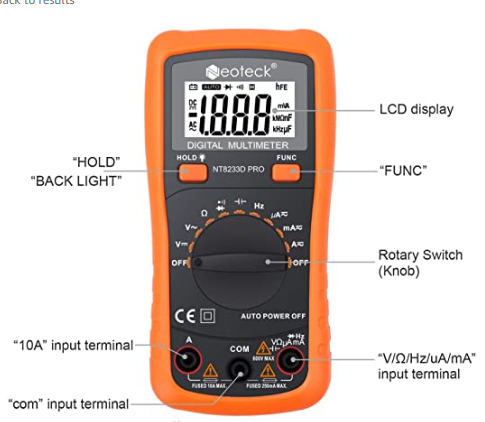
\includegraphics[ width=.6\textwidth]{handheld}
	\caption{Neoteck Handheld Digital Multi-meter}
	\label{handheld}
\end{figure}


\noindent
The multimeter is useful for probing nodes of your circuit to determine their logic level ('0' or '1'). However, depending on the situation, the logic probe or LEDs (see next section) may be more convenient.

\subsection{Using LEDs}

\noindent
An LED, as pictured in Figure~\ref{led} is a light source which will emit light if the voltage difference between the anode and cathode is high enough. For the WP7113ID LED used in the 248 labs, this voltage is 2V. In other words, if we connect the cathode to GND, and the anode to a node in our circuit, the LED will light up if the voltage of that node is at least 2V. This 'turn on' voltage for the LED is called the forward voltage. This circuit is useful to debug the circuits we breadboard, because if the node that we connect to the anode of the LED has a voltage $\ge$ 4V, the LED will light up, indicating that the node we are measuring is logic ’1’. \\

\begin{figure}[!h]
	\centering 
	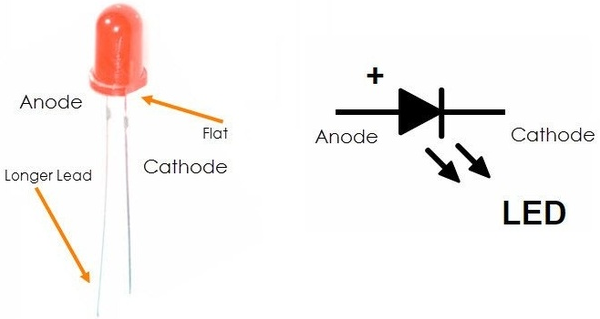
\includegraphics[ width=.5\textwidth]{led}
	\caption{Light Emitting Diode (LED)}
	\label{led}
\end{figure}

\noindent
There is one caution however. If the voltage difference between the anode and cathode is much higher than the forward voltage, the LED can become very hot and can be destroyed or even catch fire. For this reason, we have to take cautions when working on the ECEN 248 and ECEN 449/749 labs, because our VCC is much higher than 2V. This means that if we connect the anode of an LED to a node in our circuit which is logical '1' (about 5V), and the cathode to GND, the LED can easily overheat.\\

\noindent One way we can work around this problem is very simple. Instead of wiring one LED between GND and the node we are measuring, we wire two LEDs in series. This way, there is an intermediate node between GND and VCC where the cathode of the first LED meets the anode of the second, as depicted in Figure~\ref{led2}. This circuit will divide the 5V drop between the two LEDs, so that each LED only has a 2.5V drop over it. 2.5V is above the forward voltage of the LED, so it will light up, but it is not so high that it will overheat. \\

\begin{figure}[!h]
	\centering 
	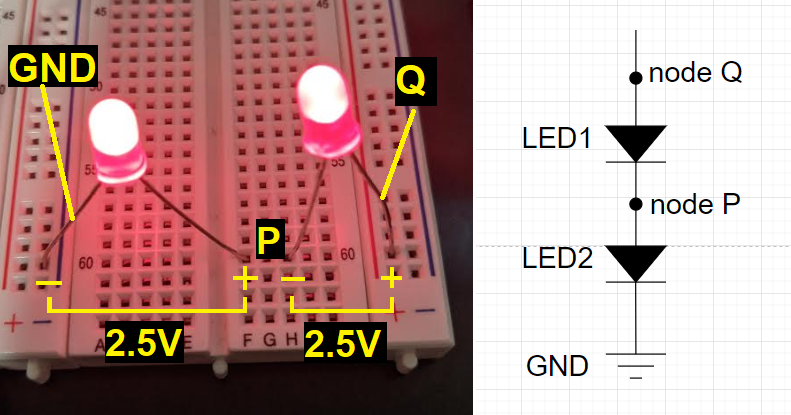
\includegraphics[ width=.6\textwidth]{led2}
	\caption{LED Voltage Divider Circuit}
	\label{led2}
\end{figure}

\noindent
The circuit in Figure~\ref{led2} acts as a simple logic probe (see next section), which will tell us if the voltage on a node in our circuit is high (logic 1) or low (logic 0). To create this simple probe circuit, simply wire two LEDs in series, as shown in Figure~\ref{led2}, and connect the cathode of LED2 to GND. Then, connect node Q to  whichever node you wish to measure. If the two LEDs light up, the voltage of the node you are measuring is high (logic 1), and if the two LEDs stay unlit, the node voltage is low (logic 0).\\

\noindent
Every time you use an LED in an ECEN 248 or ECEN 449/749 lab, be sure to use this technique!


\subsection{Using a Logic Probe}

\noindent
Another way to measure a digital voltage is to use a logic probe, as shown in Figure~\ref{probe}. Sometimes it is convenient and quick to determine the voltage of a node in a digital circuit using a logic probe, because the probe will simply tell you if the node is logic '0' or logic '1'. To use the logic probe, set the two switches to "CMOS" and "MEM" respectively. Connect the black lead of the probe to GND, and the red lead of the probe to VCC. When you touch the tip of the probe to a node in your circuit the probe will light up a different LED and make a different beep noise depending on whether you touch the tip to a node which is near VCC (logic 1) or near GND (logic 0). 
\begin{figure}[!h]
	\centering 
	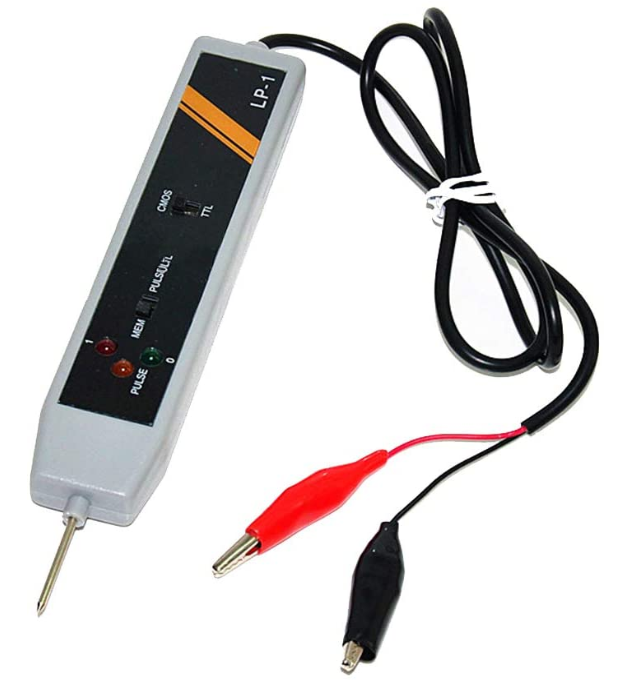
\includegraphics[ width=.5\textwidth]{probe}
	\caption{Logic Probe}
	\label{probe}
\end{figure}



\end{document}

